\section{Per-Record Replay Proportionality}
\label{sec:recovery_cost}

\begin{figure}
  \centering
  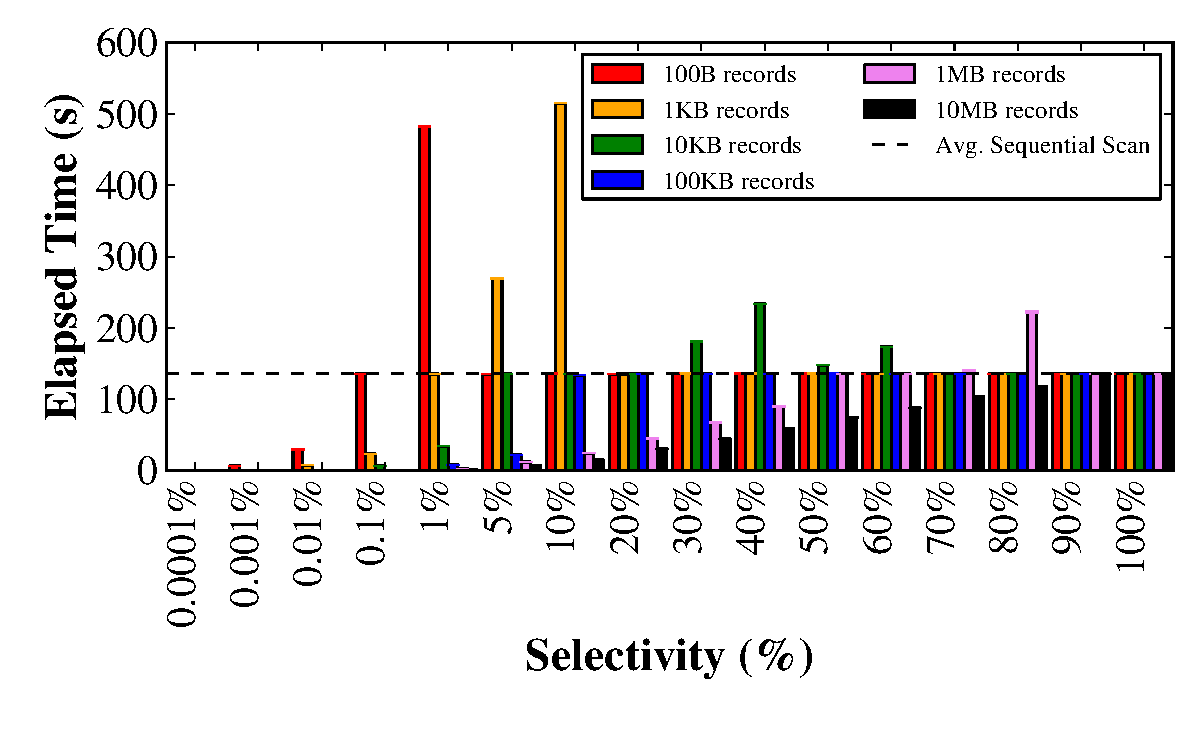
\includegraphics[width=\columnwidth]{fault_tolerance/graphs/scan_vs_seek}
  \caption{\label{fig:seek-vs-scan} Time to sequentially scan a 13.5 GB file
    vs. selectively reading a percentage of records.}
\end{figure}

\begin{figure*}
  \centering
  \begin{subfigure}[b]{\textwidth}
    \centering
    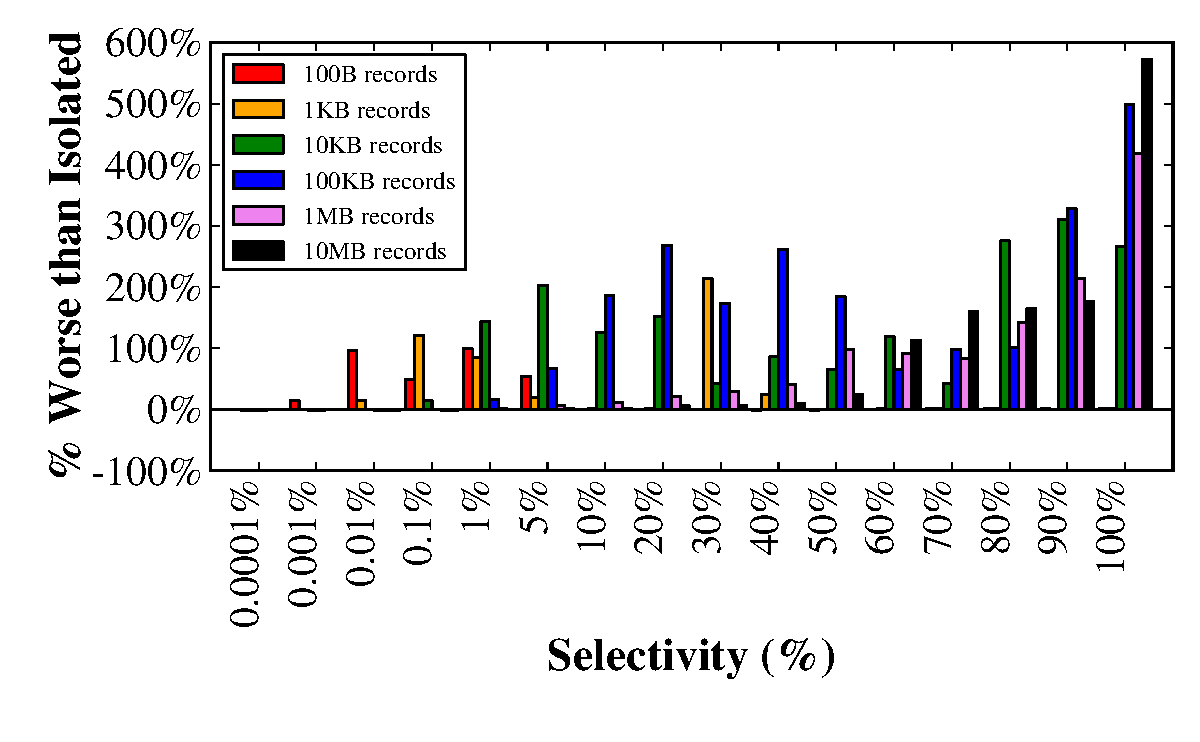
\includegraphics[width=\textwidth]{fault_tolerance/graphs/simultaneous_scan_same_file}
    \caption{\label{fig:simultaneous_same_file_scan} The effect of
      simultaneity on sequential scans.}
  \end{subfigure}
  \begin{subfigure}[b]{\textwidth}
    \centering
    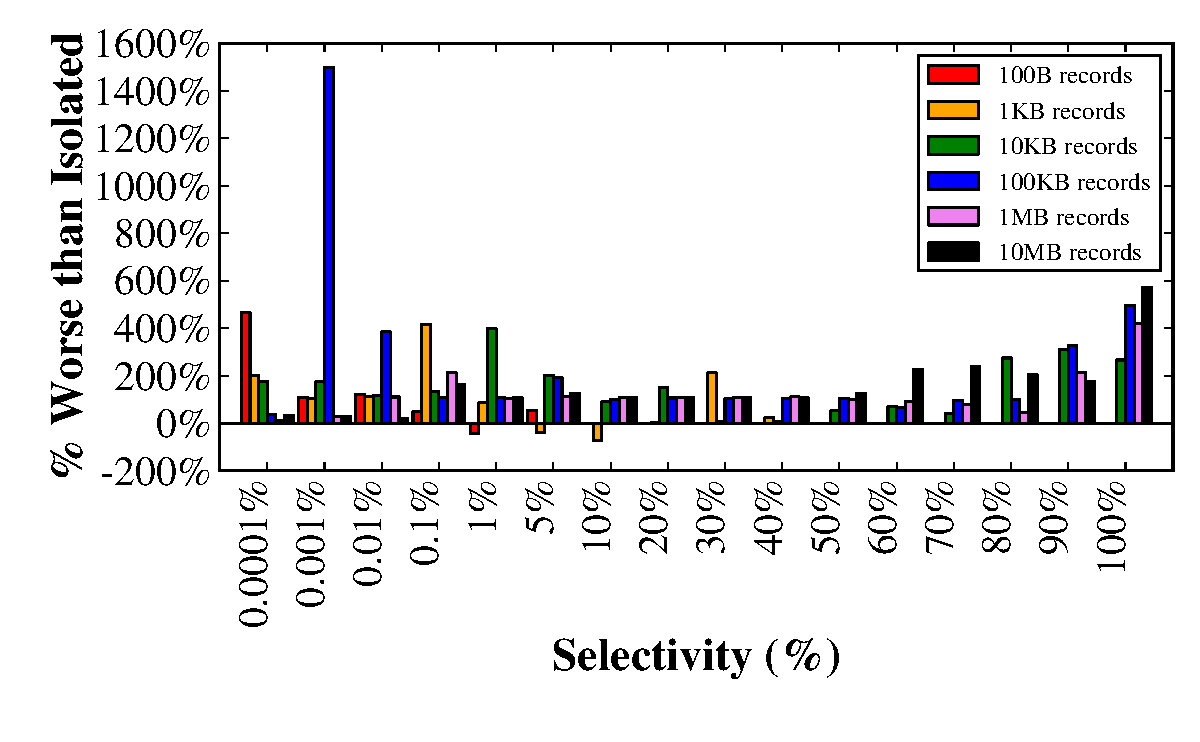
\includegraphics[width=\textwidth]{fault_tolerance/graphs/simultaneous_seek_same_file}
    \caption{\label{fig:simultaneous_same_file_seek} The effect of
      simultaneity on selective reads.}
  \end{subfigure}
  \caption{\label{fig:simultaneous_same_file} The negative impact of
    both scanning through and selectively reading from the same file simultaneously.}
\end{figure*}

\begin{figure*}
  \centering
  \begin{subfigure}[b]{\textwidth}
    \centering
    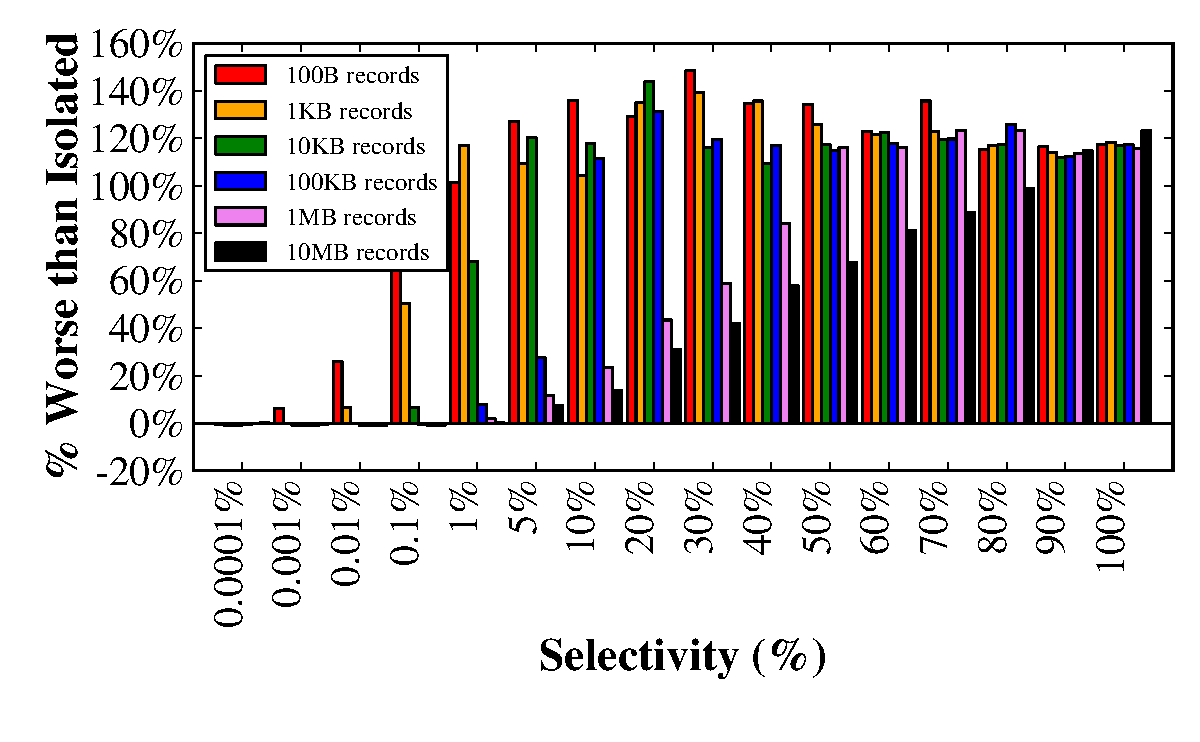
\includegraphics[width=\textwidth]{fault_tolerance/graphs/simultaneous_scan_different_files}
    \caption{\label{fig:simultaneous_different_files_scan} The effect of
      simultaneity on sequential scans.}
  \end{subfigure}
  \begin{subfigure}[b]{\textwidth}
    \centering
    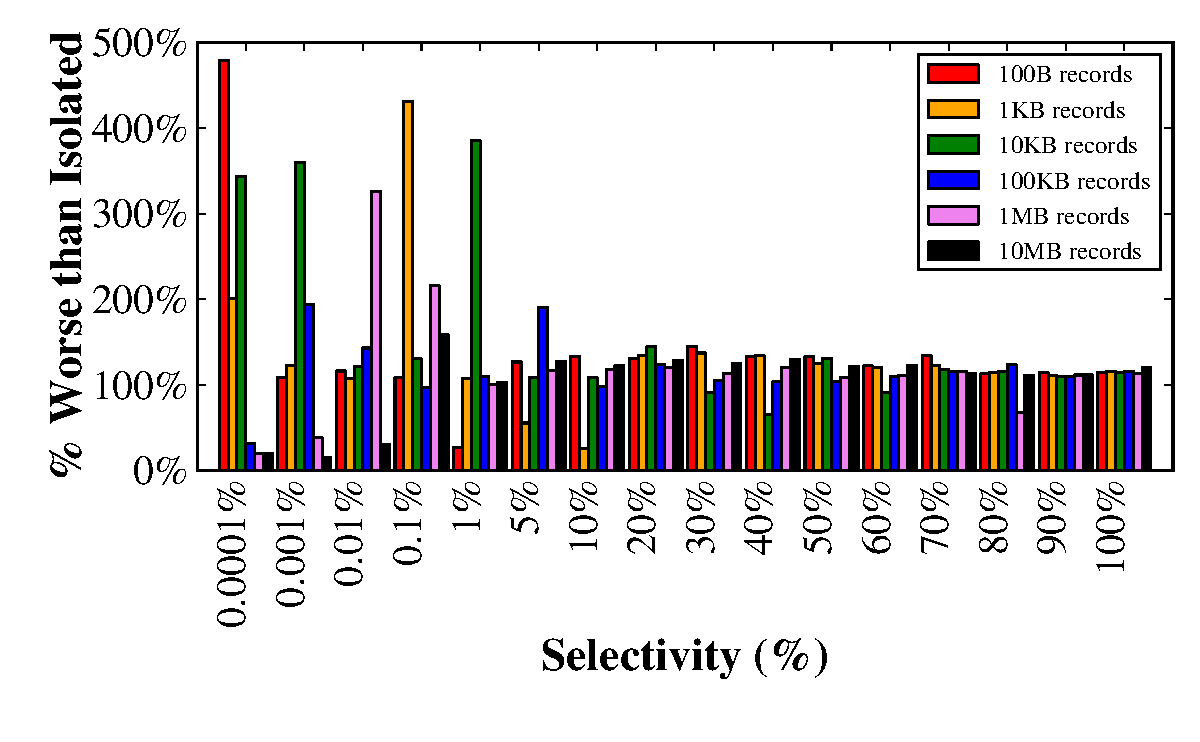
\includegraphics[width=\textwidth]{fault_tolerance/graphs/simultaneous_seek_different_files}
    \caption{\label{fig:simultaneous_different_files_seek} The effect of
      simultaneity on selective reads.}
  \end{subfigure}
  \caption{\label{fig:simultaneous_different_files} The negative impact of
    running a scan on one file while selectively reading records from a
    second file.}
\end{figure*}

When examining our options for adding fault tolerance to \themis, we were
particularly motivated by the idea of being able to recover by only reading and
re-mapping records whose intermediate data contributed to failed intermediate
partitions. We recognized that the overhead of storing this information would
potentially be quite high; in general, it requires storing information about
the lineage and intermediate partition of every intermediate
record. Nonetheless, we wanted to gain an understanding of the regimes in which
this overhead might be a reasonable tradeoff for a decreased recovery time. In
this section, we examine the potential benefits and disadvantages of this
approach using a microbenchmark.

To evaluate the potential time savings from selectively reading the subset of
input records needed to perform recovery, we created a 13.5 GB file on one of
our cluster's disks and compared the time taken to completely scan through the
file with the time taken to read a certain percentage of the file's
records. The percentage of records selectively read roughly corresponds to the
``selectivity'' of the recovery being simulated. For example, if 1\% of records
are being read, this corresponds to the amount of reading necessary to recover
from a lost of 1\% of the cluster's intermediate partitions.

As a simplifying assumption, we assumed that the records are evenly spaced
throughout the file. We completely purged the operating system's file buffer
cache and disabled any caching on our disk controllers so that each experiment
started from a cold cache.

As Figure~\ref{fig:seek-vs-scan} shows, when the selectivity of recovery is
quite small, selective reads can achieve large speedups over a sequential
scan. However, selectively reading records is far from proportional. For
example, for a file with 1KB records, the cost of sequentially scanning the
file is the same as the cost of selectively reading 1\% of its records; this
means that the loss of more than 1\% of the cluster's intermediate partitions
can be recovered from just as quickly by scanning input files as it can by
selectively reading them for I/O-bound jobs.

We suspect that this non-proportionality is due to a combination of the
overhead of seeking between records, the overhead of the relatively many
\texttt{read()} syscalls needed to retrieve those records, and the behavior of
the operating system's buffer cache. Note that for certain record sizes and
selectivities, selective reading performs dramatically worse than sequential
scanning; this is due mainly to poor interaction between the application and
the buffer cache.

In addition to its non-proportionality, selective reads have a negative impact
on the performance of other concurrent operations to the same
disk. Figure~\ref{fig:simultaneous_same_file} shows that selectively reading
from a file while scanning through it simultaneously can decrease the speed of
the scan by up to 600\%. We believe that cache interference between the two
writing processes, as well as the mechanical act of disrupting the sequentiality
of disk access with seeking, are the source of these overheads.

Figure~\ref{fig:simultaneous_different_files} shows the impact of running a
scan and a selective read over two different files on the same disk
simultaneously. Here the performance decrease for scans is much less drastic;
we believe the primary source of this performance decrease to be the overhead
imposed on the scan by disk seeks.

These results indicate, somewhat intuitively, that when the selectivity of the
recovery is very small (less than 0.01\%), it is highly beneficial to perform
selective reads. However, selective reads are only a proportional form of fault
tolerance if records are relatively large, and they have the potential to
interact poorly with other concurrent sequential scans. In addition, a recovery
with small selectivity is only likely when the cluster is fairly large, which
is a different operating environment from the ``dense'' clusters on which we
focus in this work.
